\documentclass{FEIbeamer}

\author[cferreira@fei.edu.br]{Prof. Charles Ferreira}
\title{Introdução}
\subtitle{Análise e Complexidade de Algoritmos}

\usepackage{array} % for defining a new column type
\usepackage{varwidth} %for the varwidth minipage environment
\usepackage{tikzit}
\input{uam.tikzstyles}
\setbeameroption{show notes}
\newcolumntype{M}{>{\begin{varwidth}{3cm}}l<{\end{varwidth}}} %M is for Maximal column


\lstset{morekeywords={para, ate, de, se, F1, F2, F3}}

\begin{document}

\begin{frame}[fragile]{Algoritmos}
    \question{O que são algoritmos}
\end{frame}

\begin{frame}[fragile]{Algoritmo}
    \textbf{Qualquer procedimento computacional bem definido que:}
    \bi%
    @ tenha um valor ou um conjunto de valores de entrada \ldots
    @ e produz algum valor ou conjunto de valores de saída
    \ei%
\end{frame}

\begin{frame}[fragile]{}
   \question{Como mensurar a eficiência de um algoritmo} 
\end{frame}

\begin{frame}[fragile]{Comparação}

    \textbf{Qual destes três algoritmos é o mais eficiente?}

    \triplecolumn{
        \code[size=0.5]{codes/HeapSort.p}
    }{
        \code[size=0.5]{codes/QuickSort.p}
    }{
        \code[size=0.5]{codes/bubblesort.p}
    }
\end{frame}


\begin{frame}[fragile]
\frametitle{Complexidade de Algoritmos}
% \framesubtitle{Análise de Algoritmos - Exemplo 1}
\begin{itemize}
\item Exemplo 1
\begin{lstlisting}[language=c]
#include <stdio.h>

int main(void) {
  	int count = 0;
	int i = 1;
	while(i <= 1000){
		printf("%d\n", i);
		i = i + 1;
		count = count + 1;
	}
	printf("%d\n", count);
  return 0;
}
\end{lstlisting}
\end{itemize}
\end{frame}


\begin{frame}[fragile]
\frametitle{Complexidade de Algoritmos}
\begin{itemize}
    \item Exemplo 2 
\begin{lstlisting}[language=c]
#include <stdio.h>

int main(void) {
  	int n;
	scanf("%d", &n);
	int count = 0;
	int i = 1;
	while(i <= n){
		printf("%d\n", i);
		i = i + 1;
		count = count + 1;
	}
	printf("%d\n", count);
  return 0;
}
\end{lstlisting}
\end{itemize}
\end{frame}


\begin{frame}[fragile]
\frametitle{Complexidade de Algoritmos}
\begin{itemize}
\item Exemplo 3
\begin{lstlisting}[language=c]
#include <stdio.h>

int main(void) {
	int n;
	scanf("%d", &n);
  	int count = 0;
	for(int i = 1; i <= n; i++)
		for(int j = 1; j <= n; j++)
			count = count + 1;
	printf("%d\n", count);
  	return 0;
}
\end{lstlisting}
\end{itemize}
\end{frame}

\begin{frame}[fragile]{Como ser eficiente (Exemplo)}
  \textbf{Como seria um algoritmo para buscar um valor em um vetor?}
  \bi%
  @ Qual seria a complexidade?\pause
  @@ proporcional ao tamanho do vetor\pause
  \ei
  \textbf{Agora considere que o vetor já esteja ordenado \ldots}
  \bi
  @ Faz alguma diferença?
  \ei%
\end{frame}

\begin{frame}[fragile]{Como ser eficiente (Exemplo)}
  \textbf{Demonstrando visualmente} 

  \centralize{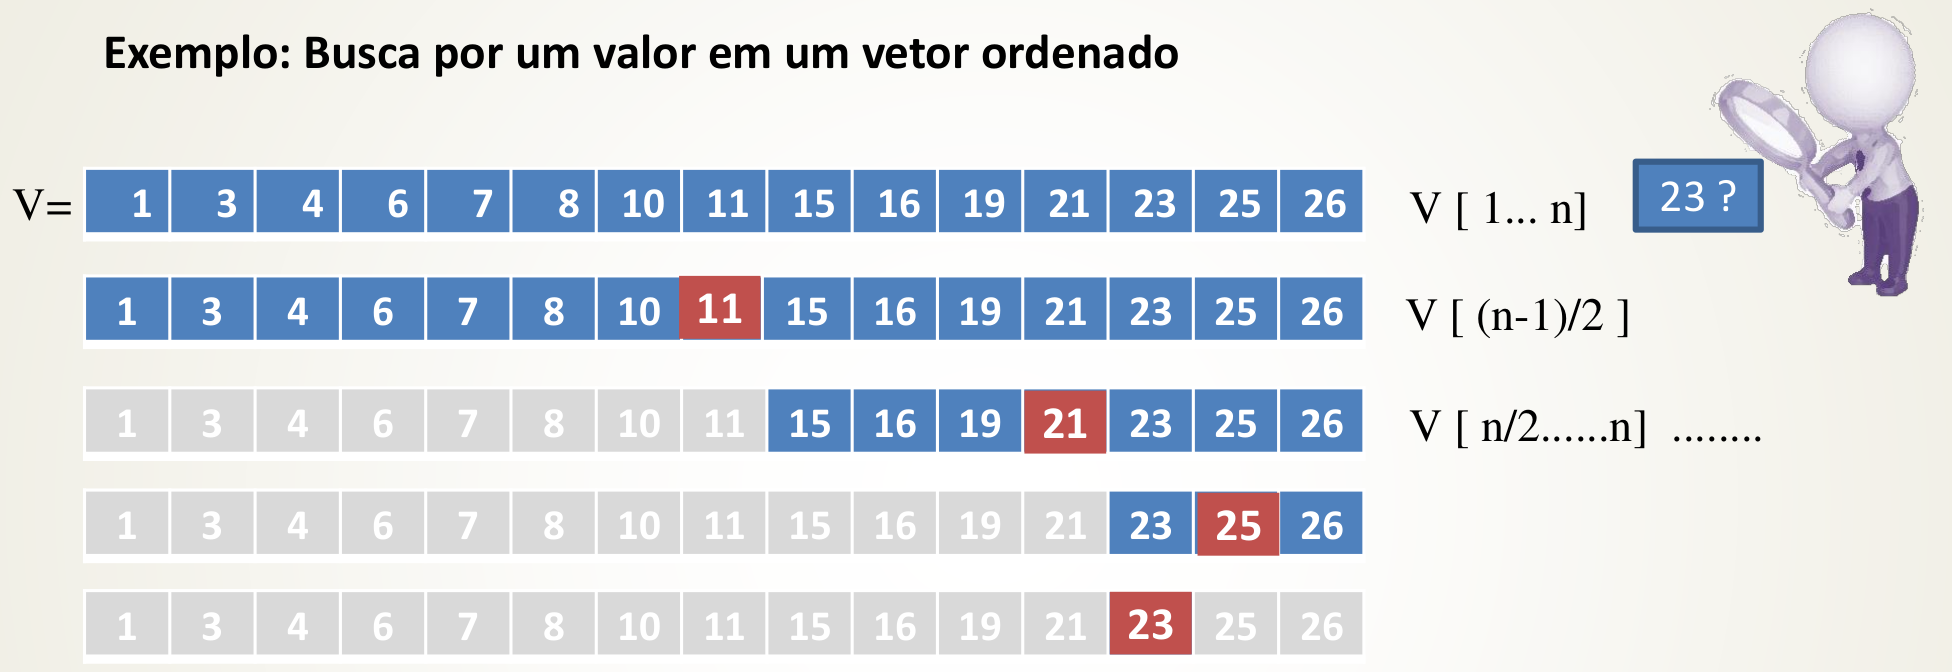
\includegraphics[width=1.0\textwidth]{images/logn1.png}}
\end{frame}


\begin{frame}[fragile]{Como ser eficiente (Exemplo)}
  \textbf{Vamos colocar alguns números \ldots}

  % \centralize{\includegraphics[width=1.0\textwidth]{images/logn2.png}}

  \begin{tabular}{lll}
    \toprule
    \textbf{Tamanho do vetor} & \textbf{Proporcional n} & \textbf{Proporcional \allbold{$\log_2n$}} \\ \midrule
    100                       & \pause 100 iterações           & \pause ~7 iterações                    \\\pause
    10.000                    & \pause 10.000 iterações        & \pause ~13 iterações                   \\\pause
    1.000.000                 & \pause 1.000.000 iterações     & \pause ~20 iterações                   \\
    \bottomrule
  \end{tabular}
\end{frame}

% \begin{frame}[fragile]{}
%   \question{Por quê a busca binária precisa apenas de \allbold{$\log_2n$} iterações}
% \end{frame}

% \note{
%   \begin{itemize}
%     \item Explicar porque a busca binária fica com complexidade de log2n
%     \item mostrar o passo a passo da demonstração
%       \Activate\doublecolumn[0.5]{%
%         \begin{align*}
%           0 &= n\\
%           1 &= n/2\\
%           2 &= n/4 = n/2^2\\
%           3 &= n/8 = n/2^3\\
%           k &= n/2^k \\
%           k &= 1 \\
%         \end{align*}
%       }{% ---------
%         \begin{align*}
%           2^k &= n\\
%           log_22^k &= log_2n\\
%           klog_22 &= log_2n\\
%           k &= log_2n
%         \end{align*}
%       }\Deactivate
%   \end{itemize}
% }


\begin{frame}[fragile]{Análise de Complexidade}
    \large
    % \bi%
    Determine a complexidade de cada um dos itens a seguir
    % \ei%
\end{frame}

\begin{frame}[fragile]{\exercise}
    \code[size=1.5]{codes/ex1.p}
\end{frame}

\begin{frame}[fragile]{\exercise}
    \code[size=1.5]{codes/ex2.p}
\end{frame}

\begin{frame}[fragile]{\exercise}
    \code[size=1.5]{codes/ex3.p}
\end{frame}

\begin{frame}[fragile]{\exercise}
    \code[size=1.5]{codes/ex4.p}
\end{frame}

\begin{frame}[fragile]{\exercise}
    \code[size=1.5]{codes/ex5.p}
\end{frame}

\begin{frame}[fragile]{\exercise}
    \code[size=1.5]{codes/ex6.p}
\end{frame}

\begin{frame}[fragile]{\exercise}
    \code[size=1.5]{codes/ex7.p}
\end{frame}

\begin{frame}[fragile]{\exercise}
    \code[size=1.5]{codes/ex8.p}
\end{frame}

\begin{frame}[fragile]{\exercise}
    \code[size=1.5]{codes/code.p}
\end{frame}

\begin{frame}[fragile]{\exercise}
    \code[size=1.5]{codes/code2.p}
\end{frame}

\begin{frame}[fragile]{\exercise}
    \code[size=1.5]{codes/code3.p}
\end{frame}

\end{document}
